\documentclass{article}
\usepackage[utf8]{inputenc}
\usepackage{graphicx}
\usepackage{hyperref}
\usepackage[bottom]{footmisc}
\usepackage{listings}
\usepackage{color}

\hypersetup{
    colorlinks=true
}
\definecolor{dkgreen}{rgb}{0,0.6,0}
\definecolor{gray}{rgb}{0.5,0.5,0.5}
\definecolor{mauve}{rgb}{0.58,0,0.82}
\lstset{
    frame=tb,
    language=R,
    aboveskip=3mm,
    belowskip=3mm,
    showstringspaces=false,
    columns=flexible,
    basicstyle={\small\ttfamily},
    numbers=none,
    numberstyle=\tiny\color{gray},
    keywordstyle=\color{blue},
    commentstyle=\color{dkgreen},
    stringstyle=\color{mauve},
    breaklines=true,
    breakatwhitespace=true,
    tabsize=3
}

\renewcommand{\contentsname}{Índice}
\renewcommand{\figurename}{Figura}

\begin{document}
\begin{titlepage}
    \centering
    
\includegraphics[width=0.5\textwidth]{images/logo-ugr.png}\par
    \vspace{1cm}
    {\Large\scshape Sistemas Inteligentes para la Gestión en la Empresa \par}
    {\huge\bfseries Pre-procesamiento de datos y clasificación binaria \par}
    \vspace{0.2cm}
    {\scshape Práctica 1 \par}
    \vfill
    {\large Víctor Vázquez Rodríguez  \par}
    {victorvazrod@correo.ugr.es \par}
    \vfill
    {\large Máster universitario en Ingeniería Informática \par}
    \vspace{0.2cm}
    {Curso 2019/20 \par}
\end{titlepage}

\tableofcontents\newpage

\section{Introducción}

Hoy en día, el procesamiento de lenguaje natural (NLP por sus siglas en inglés)
es uno de los principales campos de estudio en inteligencia artificial y
\textit{deep learning}. Este campo se centra en la interpretación del lenguaje
humano por parte de ordenadores, permitiendo cosas como el control de
dispositivos con la voz o el análisis y traducción de textos.

Un aspecto muy importante a la hora de procesar y analizar lenguaje natural es
la representación que usamos del mismo, concretamente, cómo representamos las
palabras de forma que un ordenador pueda trabajar con ellas de forma eficiente y
obtener información relevante de su significado y su contexto. Desde el punto de
vista del \textit{machine learning}, podríamos interpretar las palabras de un
texto (o de cualquier conjunto de palabras) como valores de una variable
categórica, donde cada palabra distinta supone una categoría. Uno de los métodos
más comunes y usados para representar este tipo de variables es la codificación
\textit{one-hot}, que nos permite obtener un vector de valores númericos para
cada categoría.

No obstante, esta técnica presenta grandes limitaciones para el procesamiento de
lenguaje natural, de forma que surgen los \textit{word embeddings}. Se trata de
modelos apoyados en las redes neuronales para la proyección o incrustación
(traducción literal de \textit{embedding}) de palabras en un espacio
vectorial~\cite{definition}. En la sección \ref{sec:one-hot-limitations} de este
documento se explican las limitaciones de la codificación \textit{one-hot} y
por qué son necesarios los \textit{word embeddings}, mientras que en la sección
\ref{sec:techniques} se exponen algunas de las técnicas más utilizadas. Al
final, en la sección \ref{sec:example}, se muestra un ejemplo práctico de NLP
con \textit{word embeddings}.
\newpage
\section{Exploración}
Los datos proporcionados vienen en dos tablas separadas:

\begin{itemize}
    \item La tabla \textit{identity}, que recoge información sobre
    los usuarios que realizan las transacciones (tipo de dispositivo,
    dirección, \dots).
    \item La tabla \textit{transaction}, que es la que tiene las
    transacciones como tales (tiempo, cantidad de dinero, producto
    comprado, tarjeta usada, \dots), además de la clase objetivo
    \textit{isFraud}.
\end{itemize}

Ambas tablas tienen en común un atributo \textit{TransactionID}, que usamos para
unirlas. Hay que tener en cuenta que no todas las transacciones de la tabla
\textit{transaction} tienen una identidad asociada, por lo que la unión que
realizamos es de tipo \textit{innerjoin}, quedándonos solo con los registros de
transacciones que tienen identidad.

\begin{lstlisting}
library(tidyverse)

if (!file.exists("data/train_innerjoin.csv") || !file.exists("data/test_innerjoin.csv")) {
  # Load train and test source datasets
  train_transaction <- read_csv("data/train_transaction.csv")
  train_identity <- read_csv("data/train_identity.csv")
  test_transaction <- read_csv("data/test_transaction.csv")
  test_identity <- read_csv("data/test_identity.csv")
  
  # Merge tables
  train_dataset <- merge(train_transaction, train_identity, by = "TransactionID")
  test_dataset <- merge(test_transaction, test_identity, by = "TransactionID")
  
  # Write merged datasets
  write_csv(train_dataset, "data/train_innerjoin.csv")
  write_csv(test_dataset, "data/test_innerjoin.csv")
} else {
  # Load train and test datasets
  train_dataset <- read_csv("data/train_innerjoin.csv")
  test_dataset <- read_csv("data/test_innerjoin.csv")
}
\end{lstlisting}

Como se puede apreciar en el código encargado de leer los datos y unir las
tablas, tenemos datos tanto de \textit{train} como de \textit{test}. No
obstante, los datos de \textit{test} no contienen la clase objetivo, ya que
están pensados para usarse en la competición de kaggle enviando los resultados
obtenidos de las predicciones realizadas sobre este conjunto y obteniendo las
métricas de calidad de la predicción. Como la competición ya ha finalizado, este
conjunto no nos es realmente útil, por lo que a partir de ahora trabajaremos
solo sobre el de \textit{train}.

En este conjunto de datos tenemos un total de 434 variables y 144233 registros
tras la unión de las tablas. Son muchísimos datos, por lo que tendremos que
realizar una extracción de variables para reducir su número. Si no hiciéramos
esto, los tiempos de ejecución y requisitos de memoria serían demasiado altos.
Entre estas variables tenemos la clase objetivo \textit{isFraud}, dos variables
continuas (\textit{TransactionDT} y \textit{TransactionAmt}) que tendremos que
convertir a intervalos y una serie de variables que sabemos que son categóricas
gracias a que así lo indica la competición en kaggle, ya que observando los
datos podrían parecer numéricas. Cabe destacar que, debido al carácter sensible
de los datos, el significado de muchas de las variables está enmascarado y, por
lo tanto, no podemos conocerlo.

Para conocer más información sobre los datos, usamos la función
\lstinline{df_status()} del paquete \textit{funModeling}, con la que podemos ver
el porcentaje de valores NA y la dispersión de las variables del conjunto de
datos. En la figura \ref{fig:na-barplot}, podemos ver que hay una gran cantidad
de NAs, habiendo variables con más de un 50\% de estos valores. Todas estas
variables que tienen muchos valores vacíos podremos eliminarlas en favor de otras
que tienen más información. También podemos ver, en la figura
\ref{fig:dispersity-barplot}, el porcentaje de dispersión de los valores de las
distintas variables. Se puede apreciar como hay una variable con una dispersión
extremadamente alta, que llega hasta el 80\%. Si quitamos esta variable, en la
figura \ref{fig:dispersity-reduced-barplot} vemos que también tenemos variables
con una dispersión muy baja, incluso llegando al 0\%. Todas estas variables de
dispersión elevada o muy baja las podremos eliminar del conjunto de datos.

\begin{figure}
    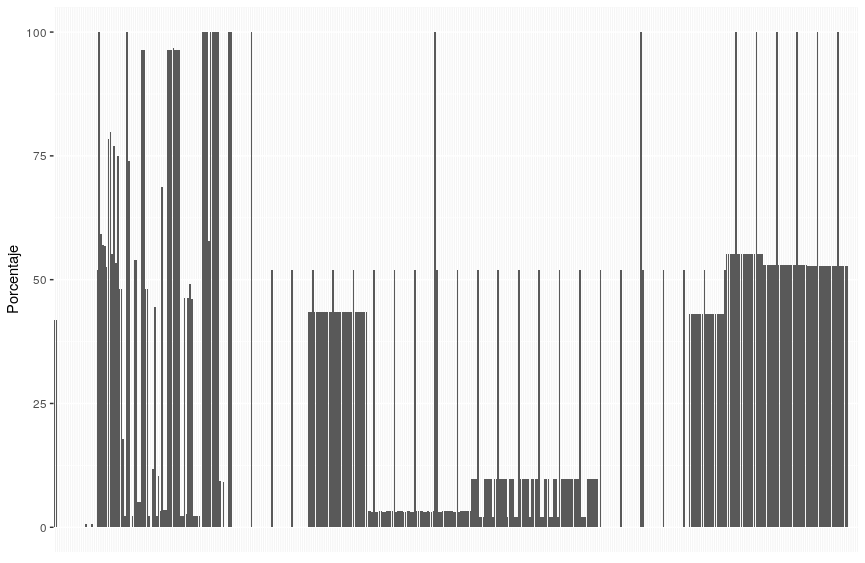
\includegraphics[width=\textwidth]{images/exploration/na-barplot.png}
    \caption{Porcentaje de valores NA por variable.}
    \label{fig:na-barplot}
\end{figure}

\begin{figure}
    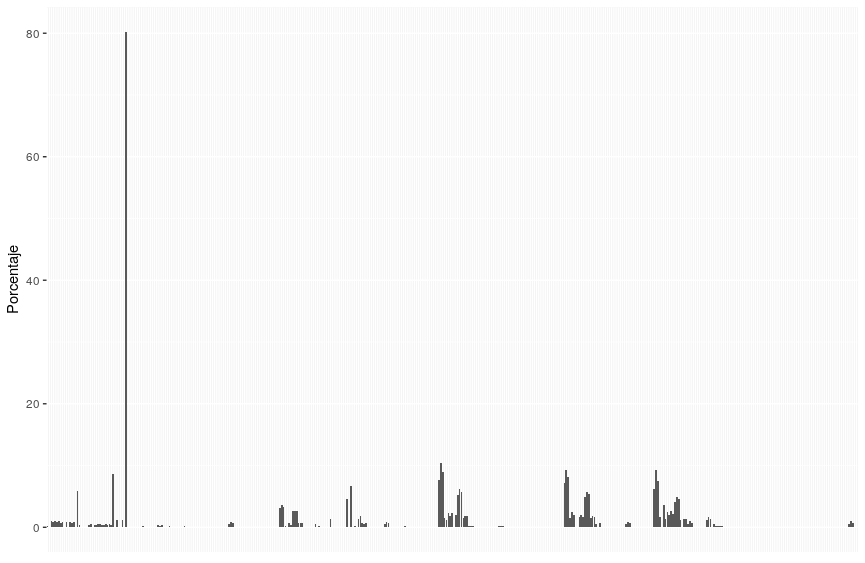
\includegraphics[width=\textwidth]{images/exploration/dispersity-barplot.png}
    \caption{Porcentaje de dispersión de valores.}
    \label{fig:dispersity-barplot}
\end{figure}

\begin{figure}
    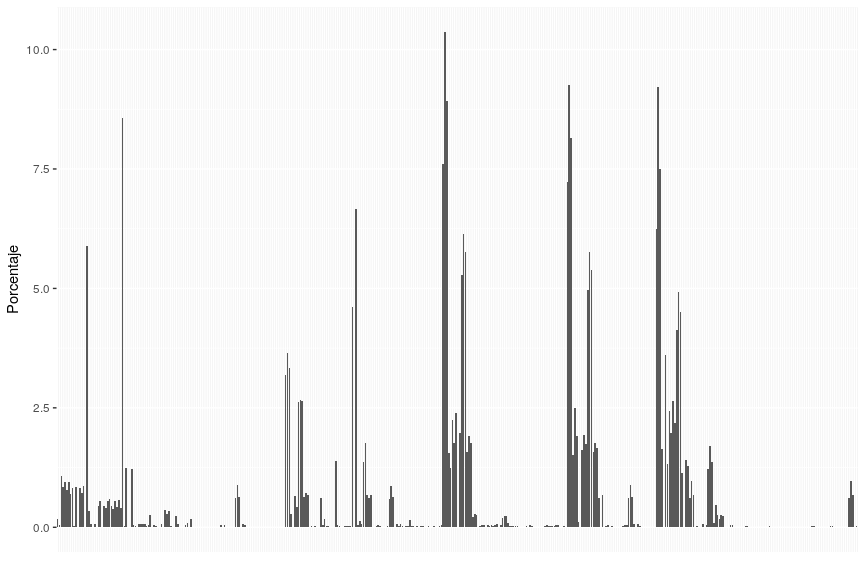
\includegraphics[width=\textwidth]{images/exploration/dispersity-reduced-barplot.png}
    \caption{Porcentaje de dispersión de valores para variables con dispersión inferior al 60\%.}
    \label{fig:dispersity-reduced-barplot}
\end{figure}

También podemos fijarnos en la correlación entre variables para ver si hay
algunas que podamos eliminar. Si dos variables están muy correladas, podremos
eliminar una de ellas, ya que ambas nos aportarían la misma información. En la
figura \ref{fig:correlation-heatmap} tenemos un mapa de calor que refleja las
correlaciones entre las variables de tipo numérico del conjunto de datos. Las
zonas con un tono más claro indican una alta correlación, por lo que serían
pares de variables a considerar.

\begin{figure}
    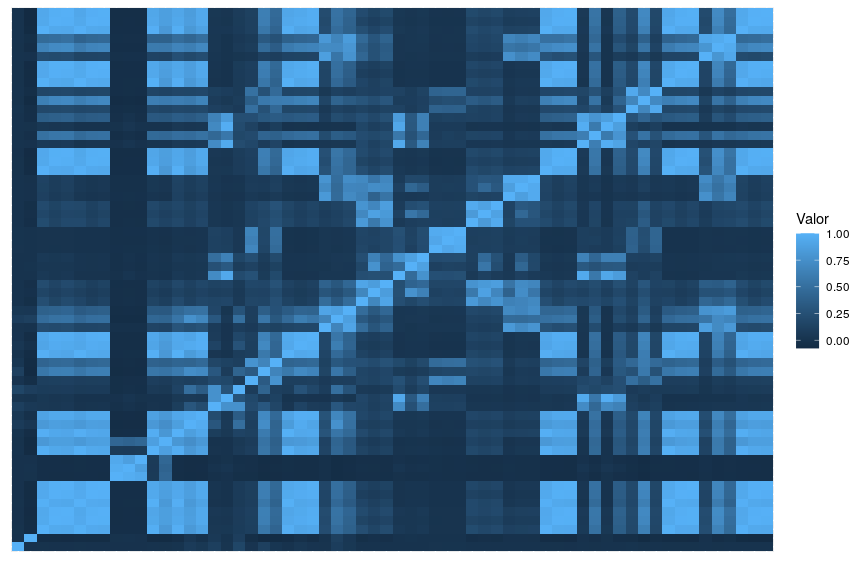
\includegraphics[width=\textwidth]{images/exploration/correlation-heatmap.png}
    \caption{Correlación entre variables numéricas.}
    \label{fig:correlation-heatmap}
\end{figure}

Para terminar con la exploración, podemos observar el número de registros
que tenemos para cada valor de la clase objetivo \textit{isFraud}, lo cuál
podemos ver en la figura \ref{fig:class-barplot}. Como era de esperar, hay
muchos más ejemplos de transacciones que no son fraude que de las que sí lo son,
ya que estas últimas son menos frecuentes. Para entrenar los clasificadores,
necesitaremos balancear el conjunto de datos primero.

\begin{figure}
    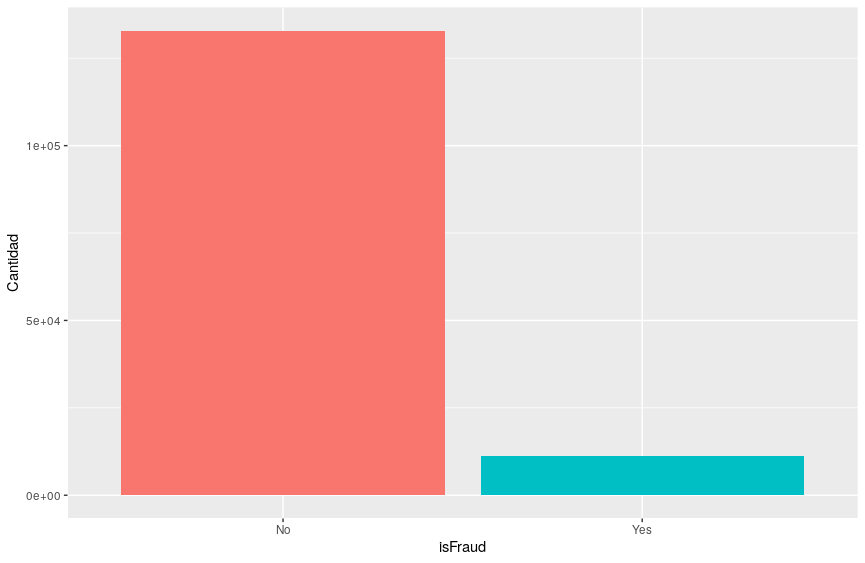
\includegraphics[width=\textwidth]{images/exploration/class-barplot.png}
    \caption{Cantidad de ejemplos de cada valor de la clase objetivo presentes en el conjunto de datos.}
    \label{fig:class-barplot}
\end{figure}
\newpage
\section{Pre-procesamiento}

Antes de poder entrenar los clasificadores con los datos, se deben realizar
algunas tareas de pre-procesamiento. Para empezar, observamos que las clases no
están balanceadas, teniendo unos 680.000 positivos y alrededor de 1.300.000
negativos. Por ello, aplicamos \textit{undersampling} para balancear las clases
obteniendo la proporción de registros positivos sobre el total y haciendo
\texttt{sample} de los registros negativos para obtener la misma proporción, tal
y como se puede ver en el fragmento de código siguiente:

\begin{lstlisting}
positives = data.filter(data["class"] == 1)
negatives = data.filter(data["class"] == 0)
ratio = float(positives.count()) / float(data.count())
sampled_negatives = negatives.sample(False, ratio)
data = positives.union(sampled_negatives)
\end{lstlisting}

También tenemos que dividir el conjunto de datos en las particiones para
entrenamiento y prueba, que conseguimos con la función \texttt{randomSplit} de
Spark. En mi caso, he decidido usar un 70\% de los registros para entrenamiento
y el resto para prueba.

Una vez realizadas estas dos tareas, ya podríamos entrenar los modelos. No
obstante, tenemos que tener en cuenta que los clasificadores toman como entrada
un vector de características, no una serie de columnas. Spark nos proporciona
\texttt{VectorAssembler} para crear juntar las columnas deseadas en un vector y
colocarlo en una nueva columna del conjunto de datos. Hay otro impedimento, y es
que la columna \textit{PredSS\_central\_2} contiene caracteres de texto, los
cuales no acepta \texttt{VectorAssembler}. Usamos entonces
\texttt{StringIndexer} para convertir estos caracteres en valores numéricos que
si pueden incorporarse a los vectores de características. Tanto
\texttt{StringIndexer} como \texttt{VectorAssembler} se colocan en un
\texttt{Pipeline} de Spark al que luego se añaden los distintos clasificadores.
Estos \textit{pipelines} permiten entrenar los flujos de procesamiento completos
para los datos, obteniendo modelos que trabajan directamente sobre los conjuntos
de datos sin tener que realizar cada etapa de forma manual.

\begin{lstlisting}
def create_preprocess_pipeline():
    si = StringIndexer(
        inputCol="PredSS_central_2",
        outputCol="PredSS_central_2_indexed"
    )

    va = VectorAssembler(
        inputCols=["PSSM_r2_-3_S", "PSSM_central_0_P",
            "PSSM_r1_1_Y", "PSSM_r1_-3_R", "PSSM_r1_0_R",
            "PredSS_central_2_indexed"],
        outputCol="features"
    )

    return Pipeline(stages=[si, va])
    \end{lstlisting}
\newpage
\section{Clasificadores}
Como clasificadores, he decidido entrenar modelos de regresión logística y
perceptrón multicapa. Cabe destacar que he intentando entrenar otros modelos
como \textit{Random Forest} o SVM, pero era incapaz de ello ya que RStudio se
encontraba siempre con algún error fatal que hacía abortar la sesión.

En las siguientes secciones, se va a explicar cómo se ha llevado a cabo el
entrenamiento de los modelos usando el paquete \textit{caret} y, también, se
compararán los resultados de cada uno para cada conjunto de datos de los dos que
hemos preparado.

Antes de entrenar cualquier modelo, los datos se dividen en dos subconjuntos
para entrenamiento y validación usando la función
\lstinline{createDataPartition()} de \textit{caret}. En mi caso, un 70\% se
destina a entrenamiento y, el resto, a validación.

\begin{lstlisting}
library(caret)

set.seed(0)

# ROSE
train_index_rose <- createDataPartition(data_balanced_rose$isFraud, p = .7, list = FALSE)
train_rose <- data_balanced_rose[train_index_rose, ]
val_rose <- data_balanced_rose[-train_index_rose, ]

# SMOTE
train_index_smote <- createDataPartition(data_balanced_smote$isFraud, p = .7, list = FALSE)
train_smote <- data_balanced_smote[train_index_smote, ]
val_smote <- data_balanced_smote[-train_index_smote, ]
\end{lstlisting}

\subsection{Regresión logística}
A pesar de su nombre, la regresión logística es una técnica muy utilizada en
problemas de clasificación binaria, como es el caso del nuestro. Esta técnica se
apoya en la función sigmoide, la cuál nos proporciona un valor entre 0 y 1, que
interpretamos como la probabilidad de que se pertenezca a la clase principal.

He decidido usar este clasificador debido a que es muy simple y no requiere de
un gran consumo de recursos, lo cuál favorece su entrenamiento en mi ordenador
personal, donde se ha realizado la práctica.

\begin{lstlisting}
# ROSE
lr_grid_rose <- expand.grid(.nIter = 5)
lr_control_rose <- trainControl(method = "repeatedcv", number = 10, repeats = 5)
lr_model_rose <- train(
  isFraud ~ .,
  data = train_rose,
  method = "LogitBoost",
  trControl = lr_control_rose,
  tuneGrid = lr_grid_rose
  )

lr_prediction_rose <- predict(lr_model_rose, val_rose, type = "raw")

# SMOTE
lr_grid_smote <- expand.grid(.nIter = 5)
lr_control_smote <- trainControl(method = "repeatedcv", number = 10, repeats = 5)
lr_model_smote <- train(
  isFraud ~ .,
  data = train_smote,
  method = "LogitBoost",
  trControl = lr_control_smote,
  tuneGrid = lr_grid_smote
)

lr_prediction_smote <- predict(lr_model_smote, val_smote, type = "raw")
\end{lstlisting}

Como se puede ver en el código, los clasificadores de regresión loǵistica se han
entrenado usando 5 iteraciones. Además, se ha aplicado validación cruzada con 10
árboles y otras 5 repeticiones. Las medidas de calidad obtenidas para las
predicciones realizadas sobre los conjuntos de validación se pueden ver en la
figura \ref{fig:lr-barplot}.

En el caso concreto de nuestro problema, el \textit{recall} o exhaustividad es
una medida muy importante, ya que un falso negativo (una transacción fraudulenta
no identificada como tal) es muy costoso. Como se puede ver, esta medida no es
especialmente buena para la predicción realizada por estos modelos.

Apreciamos que las medidas son prácticamente idénticas para ambos conjuntos de
datos, siendo las del clasificador aplicado al conjunto de SMOTE ligeramente
mejores. Podemos asumir entonces que la aplicación de las técnicas no ha tenido
un impacto relevante en los resultados.

\begin{figure}
    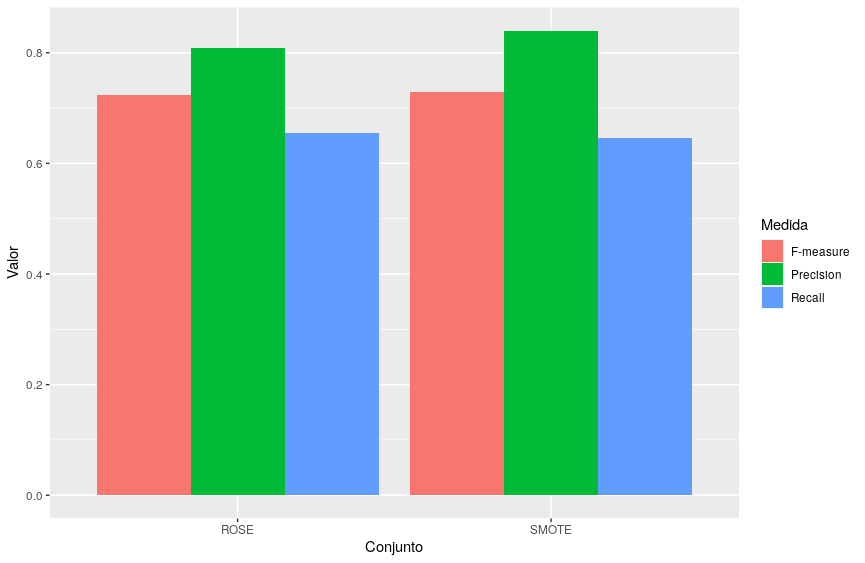
\includegraphics[width=\textwidth]{images/classification/lr-barplot.png}
    \caption{Medidas de calidad de la predicción realizada mediante regresión logística.}
    \label{fig:lr-barplot}
\end{figure}

\subsection{Perceptrón multicapa}
El segundo clasificador utilizado es el perceptrón multicapa. Estas redes
neuronales son ampliamente utilizadas en problemas de clasificación debido a su
capacidad para extraer características ocultas de los patrones del conjunto de
entrenamiento.

\begin{lstlisting}
# ROSE
mlp_control_rose <- trainControl(method = "repeatedcv", number = 10, repeats = 5)
mlp_model_rose <- train(
  isFraud ~ .,
  data = train_rose,
  method = "mlp",
  trControl = mlp_control_rose
)

mlp_prediction_rose <- predict(mlp_model_rose, val_rose, type = "raw")

# SMOTE
mlp_control_smote <- trainControl(method = "repeatedcv", number = 10, repeats = 5)
mlp_model_smote <- train(
  isFraud ~ .,
  data = train_smote,
  method = "mlp",
  trControl = mlp_control_smote
)

mlp_prediction_smote <- predict(mlp_model_smote, val_smote, type = "raw")
\end{lstlisting}

Es cierto que consumen más recursos que el otro clasificador usado, pero también
se podría esperar que se consiguieran resultados más precisos. En la figura
\ref{fig:mlp-barplot} se pueden ver estos resultados, que son incluso peores que
los obtenidos por el clasificador basado en regresión logística. Sí que podemos
destacar los resultados obtenidos para el conjunto de datos balanceado con
SMOTE. En este caso, vemos como la precisión es muy baja y la exhaustividad es
muy elevada. El clasificador es capaz de identificar muy bien los verdaderos
positivos del conjunto, pero también cuenta con un gran número de falsos
positivos. En resumen, sacamos de aquí que este clasificador tiende a clasificar
como fraude la mayoría de las transacciones.

\begin{figure}
    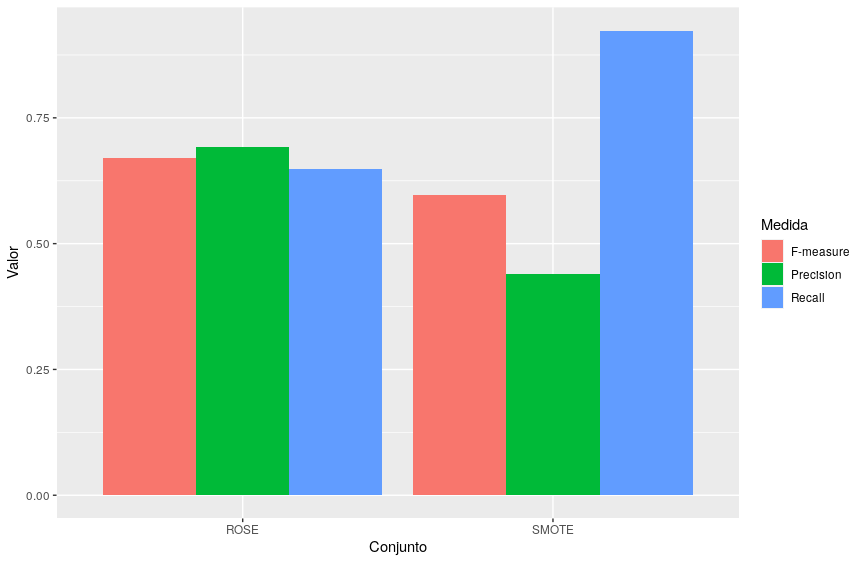
\includegraphics[width=\textwidth]{images/classification/mlp-barplot.png}
    \caption{Medidas de calidad de la predicción realizada por el perceptrón multicapa.}
    \label{fig:mlp-barplot}
\end{figure}

\subsection{Comparación}
Para comparar los clasificadores entre ellos, vamos a separar los resultados
obtenidos para el conjunto de datos al que se ha aplicado ROSE y al que se ha
aplicado SMOTE.

En la figura \ref{fig:rose-barplot}, tenemos los resultados de ambos
clasificadores sobre el conjunto de validación de ROSE. Apreciamos claramente
como la precisión ha sido menor con el perceptrón multicapa, mientras que la
exhaustividad se ha mantenido practicamente igual. En definitiva, los resultados
dados por el perceptrón han sido peores que los obtenidos con la regresión
logística.

En cuanto al conjunto de SMOTE, podemos ver los resultados de ambos
clasificadores en la figura \ref{fig:smote-barplot}. Aquí es donde tenemos los
resultados más dispares. Ya hemos explicado en el apartado anterior que los
resultados del perceptrón nos hacen ver que clasifica la mayoría de
transacciones como fraudulentas, lo que hace que no sea un clasificador fiable.
La regresión logística vuelve a ser mejor que el perceptrón, aunque sus
resultados tampoco son demasiado buenos.

\begin{figure}
    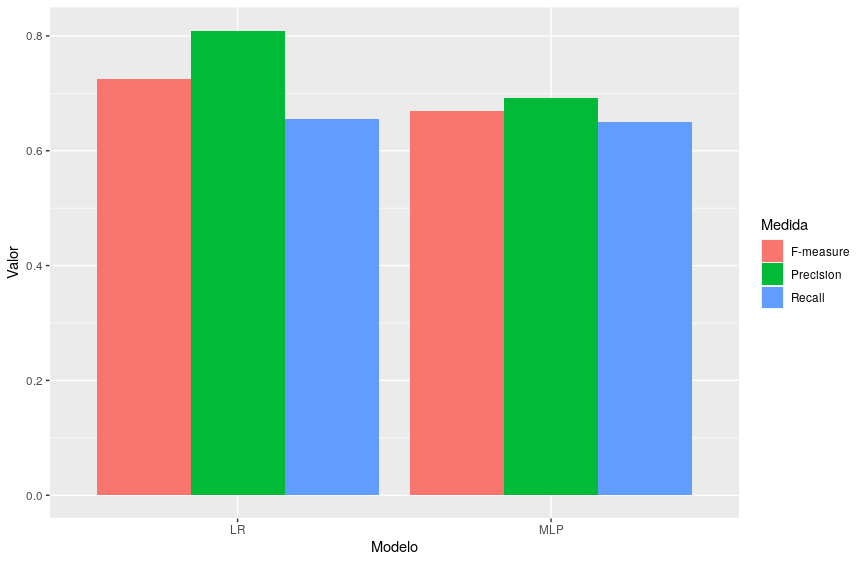
\includegraphics[width=\textwidth]{images/classification/rose-barplot.png}
    \caption{Medidas de calidad de las predicciones realizadas sobre el conjunto de datos ROSE.}
    \label{fig:rose-barplot}
\end{figure}

\begin{figure}
    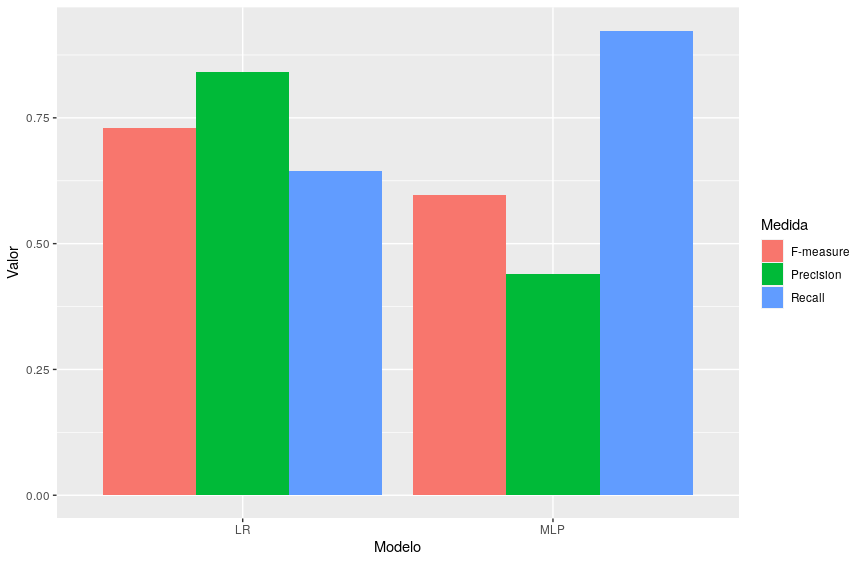
\includegraphics[width=\textwidth]{images/classification/smote-barplot.png}
    \caption{Medidas de calidad de las predicciones realizadas sobre el conjunto de datos SMOTE.}
    \label{fig:smote-barplot}
\end{figure}
\newpage
\section{Conclusiones}

En este proyecto se han realizado muchas pruebas y se ha obtenido una gran
cantidad de datos, de los cuáles se pueden extraer algunas conclusiones. La
primera que salta a la vista viendo los tiempos de respuesta de los contenedores
en ejecución, es que las aplicaciones contenerizadas pueden ser aptas para
restricciones de tiempo real. En esta línea, si volvemos a observar los datos
del cuadro \ref{tab:response-results}, la desviación típica en los tiempos en
i386 es considerablemente inferior a la que se aprecia en arm32v7 en cualquiera
de las situaciones (en ejecución, parado o pausado). En los tiempos de
lanzamiento también se aprecia ésto, aunque la diferencia de desviaciones es
menor, tal y como se ve en el cuadro \ref{tab:start-results}. Podríamos concluir
entonces que i386 ofrece un comportamiento más determinista que arm32v7, al
menos en los dispositivos usados.

Por otra parte, considero que los tiempos de lanzamiento que se han registrado
son demasiado elevados para sistemas con restricciones de tiempo real "duras",
aunque sí podrían ser aptos para los que tengan restricciones "blandas". El
principal problema lo encontramos en la poca consistencia de tiempos en todas
las tareas de gestión de los contenedores, tal y como se aprecia en los
resultados de los tiempos de respuesta para los contenedores parados y pausados
y de los tiempos de lanzamiento.

En definitiva, considero que los resultados son esperanzadores para la
aplicación de las tecnologías de contenerización a la automatización de la
industria, aunque creo que sería necesario construir herramientas específicas
para este caso de uso, como pueden ser motores y orquestadores de contenedores
que tengan en cuenta y garanticen los requisitos de tiempo de cada aplicación
contenerizada. Además, la plataforma de ARM necesita de mejoras en el campo del
trabajo con contenedores para poder ser una opción fiable.
\newpage
\end{document}
